\section{YOLO9000 (YOLOv2)}  \label{sec:yolov2}

YOLO9000, also known as YOLOv2, is an improvement of the YOLOv1 model \cite{yolo9000_2017}. The real time object detection model YOLOv2 is first introduced in 2016. The name YOLO9000 is stem from the fact that the model is capable of detecting over 9,000 object categories in real-time,  which is significantly more than the original YOLO model. This is achieved by finetunning the model with the WordNet language database, which also is the database that ImageNet labels set pulls from.

\subsection{Accuracy Improvement}
The YOLOv2 model propose five changes that improve the accuracy of YOLOv1. The first change is the addition of \textbf{batch normalization} on convolutional layer, which improve YOLOv1 mAP score by more than 2\%. Batch normalization remove the need of dropout technique \cite{dropout_2014}, which drop certain activated neuron to avoid overfiting problem \cite{szeliski_cv_book}. The second change is utilize \textbf{higher resolution classifier}. While YOLOv1 only train on $224 \times 224$ images for classification task, YOLOv2 further train the classifier with $448 \times 448$ images. The higher resolution classifier increase the YOLOv1 mAP score by 4\%. The third change is the use of \textbf{passthrough layer}. Since convolutional layer decrease the image spatial dimension gradually, thus it become more diffcult to detect smaller object in the image as more convolutional layers are used. For this reason, the passthrough layer help bring the image detail from the higher spatial dimension to the lower spatial dimension map, simmilar to skip connection in ResNet \cite{resnet_2016}.

Since each divided cell in YOLOv1 only predict exactly 2 bounding boxes, 1 confidence score, and 1 classification label (the highest probability class), thus the model has poor performance in detecting object appear near together, especially small object. To address this problem, YOLOv2 model propose the fourth and fifth change. 

The fourth change is utilizing \textbf{anchor boxes} at each cell instead of randomly initialize bounding box like in YOLOv1. The size and aspect ratio of the anchor box is heavily depend on the domain that the model will be applied to. For example, when apply the model to traffic detection task, then the main shape and size the model need to look for are pedestrian and different vehicle. Thus starting the anchor box at these shape and size improve the runtime for both training and inference. For this reason, a k-means clustering algorithm is used to find the top-k common dimension in the training set \cite{yolo9000_2017}. The anchor boxes is then used to predict the bounding box. The YOLOv2 model predict 5 parameters for each bounding box $[t_x, t_y, t_w, t_h, and t_o]$, where $t_x, t_y$ and $t_w, t_h$ are center and dimention of the bounding box in relation to the cell and the image dimention, respectively. These 5 parameters are the same as the prediction make by YOLOv1. Given that the cell is $(c_x, x_y)$ offset from the top-left conner of the image, and the anchor box have the dimension of $p_w, p_h$, then the predicted bounding box  has the center at $(b_x, b_y)$ with dimension of $b_w, b_h$, and can be computed with constraint by sigmoid function, as shown in Firgure \ref{fig:yolov2_bbox}.

\begin{figure}[!ht]
    \centering
    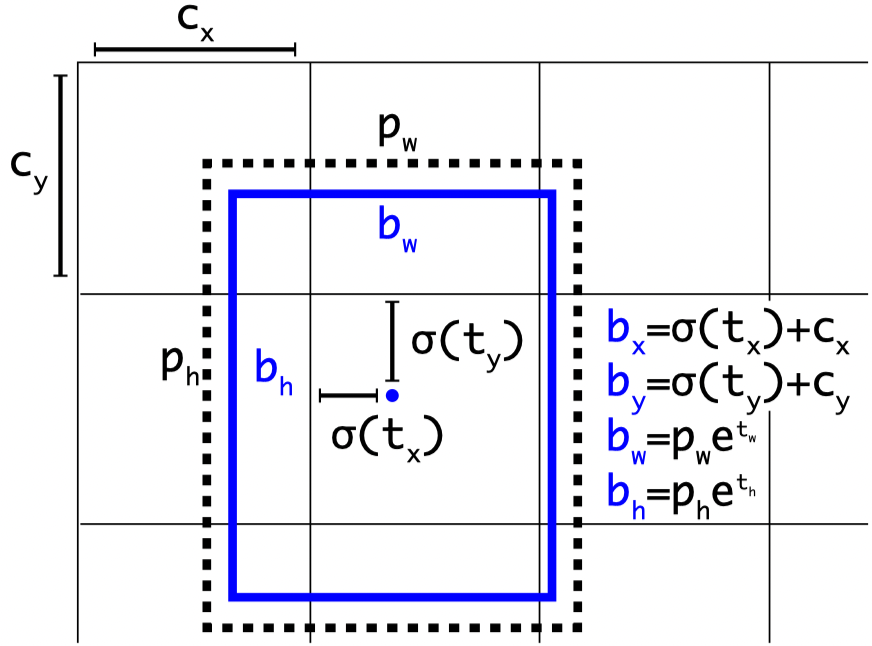
\includegraphics[width=3in]{figures/yolov2_bbox.png}
    \caption{YOLOv2 bouding box (in blue) generation offset from the anchor box (in black) \cite{yolo9000_2017}} 
    \label{fig:yolov2_bbox}
\end{figure}

Since the anchor boxes is used to predict the bounding box, thus remove the need of the fully connected layer. In addition to the removal of fully connected layer, YOLOv2 model also move the classification label from cell level to anchor box level. In other words, YOLOv2 model predict a classification label for each anchor box \cite{yolo9000_2017}. Let the image be divided to an $S \times S$ cell grid, each cell generate $B$ anchor boxes, and the dataset have $C$ catagorise, then the image detection is encoded as a $S \times S \times B*(4+1+C)$ tensor. The achor box scheme remove the assumption of one object per grid cell and improve the mAP score by 5\% approximately.

The fifth change is \textbf{multi-scale training}. Since YOLOv2 remove the fully connected layer, thus it can process the image of any size. Therefore, instead of training with a fixed size, the model choose a new input image dimension every 10 batches. Additionally, since the model is downsample by 32 times during it process, to avoid quantization, the input image should be a multiple of 32: {320, 352, ..., 608}. This trainning scheme force the model to be able to predict object at different resolution, which train the network to predict object of different scale.

\subsection{Runtime Improvement}
The YOLOv2 further simplify the archietecture used in YOLOv1. The YOLOv2 model use a new classification model, namely Darknet-19. The overall archietecture of Darknet-19 is shown in Firgure \ref{fig:darknet19_archite}. Compare to the GoogLeNet, Darknet-19 is smaller with 5.58 billion operations instead of 8.52 billion operations, while have higher top-5 accuracy in classification task after training \cite{yolo9000_2017}.Compare to YOLOv1's CNN archietecture, Darknet-19 only has 19 convolutional layers and 5 max-pooling layers, while YOLOv1's CNN consist of 24 convolutional layers, 4 max-pooling layers, and 2 fully connected layers. The Darknet-19 is first trained with the ImageNet 1000 for classification task. The Darknet-19 model is then adapted for object detection task by replacing the last convolutional layer with three $3 \times 3$ convolutional layer that output 1024 channels, folowed by $1 \times 1$ convolutional layer to convert $S \times S \times 1024$ to $S \times S \times B*(4+1+C)$.

\begin{figure}[!ht]
    \centering
    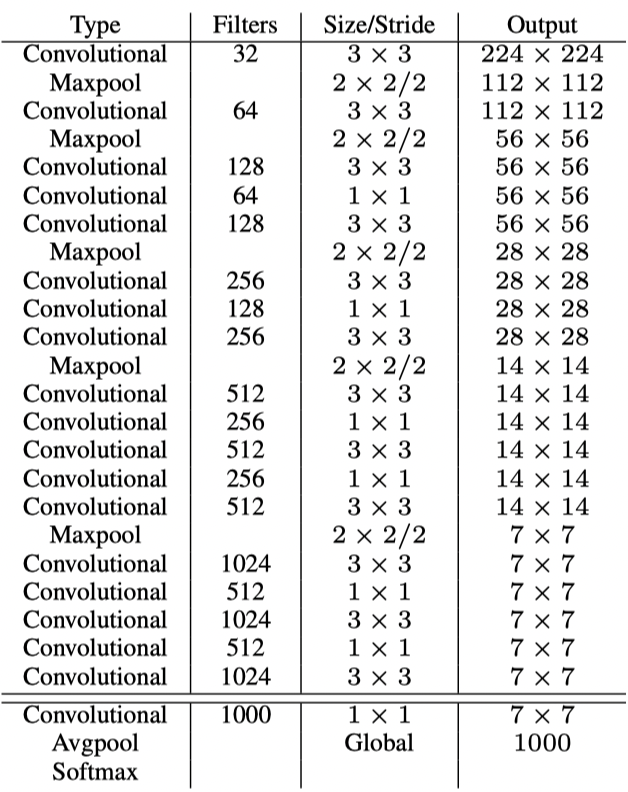
\includegraphics[width=4in]{figures/darknet19_archite.png}
    \caption{Darknet-19 architecture \cite{yolo9000_2017}} 
    \label{fig:darknet19_archite}
\end{figure}